\section{Clustering}
Describe the clustering procedure--refer to ISRR when needed.


\begin{figure*}[!t]
\centering
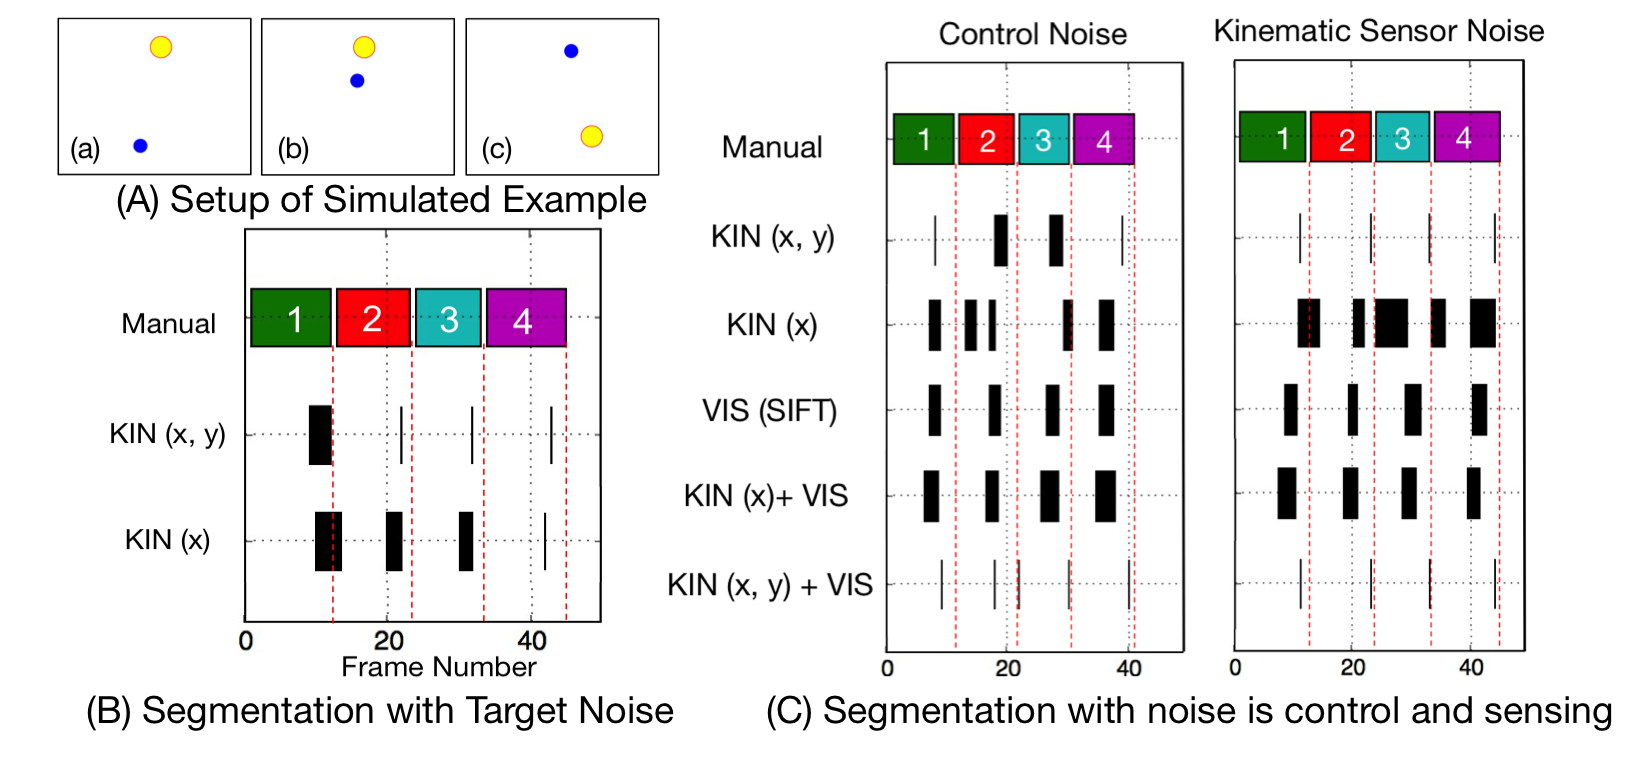
\includegraphics[width=0.8\linewidth]{figures/toyEx}
\caption{Each row is a sequence of transitions represented by blocks. The width of every block represents the confidence interval conveying the length of transition, with some transitions being sharp while others are longer.}
\label{fig:toyEx}
\vspace{-15pt}
\end{figure*}